
\chapter{Einführung}
\section{Einleitung, Ziele und Vorgehensweise}
 

Die vorliegende Diplomarbeit entstand im Rahmen  der Forschungstätigkeit am Institut für Tragwerkplanung und Ingenieurholzbau. Sie schließt an die Arbeiten von  Kirchmayer [1] \cite{1} und  Schernberger [2] an. Im Rahmen des Forschungsprojektes "`Weitgespannte Flachdeckensysteme in Holzspanbeton – Verbundweise"'  sind ihre Arbeiten entstanden. Die Ausarbeitung von Schernberger befasst sich mit der allgemeinen Anwendung und den Einsatzgebieten des Holzleichtbetons. Kirchmayer hat anhand von Versuchsreihen das Tragverhalten- und Verformungsverhalten verschiedener Aufbauten und Verbindungsmittel untersucht.  Durch diese Versuche und Analysen ist der dargestellte Sandwichaufbau \ref{sandwich} entstanden. 



\begin{figure}[h!]
\begin{center}
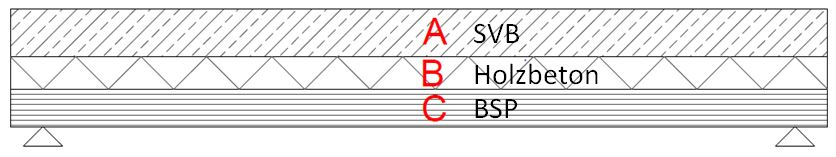
\includegraphics[scale=0.7]{Einleitung/sandwichaufbau.JPG}
\caption{Sandwichaufbau}
\label{sandwich}
\end{center}
\end{figure}

\subparagraph{Ziele und Vorgehensweise:}

Das erste übergeordnete Ziel dieser Arbeit ist die Entwicklung eines Sandwichaufbaus aus Brettsperrschichtholz (BSP), Holzleichtbeton und selbeverdichtendem Beton\,(SVB). Der SVB nimmt in dem Aufbau die Druckschicht ein, das BSP die Zugschicht und der Holzleichtbeton die Mittelschicht. Die Verbindung der unterschiedlichen Werkstoffe wird durch die Anwendung von Schrauben und einem Kleber gewährleistet. Das zweite Ziel dieser Arbeit ist die Nachrechnung der Versuchsergebnisse mit den „$\gamma$ -Verfahren“ und dem Finite Elemente Programm „Sofistik“. Es sollen die Grundlagen zur Bemessung des Sandwichaufbaus entwickelt werden. 
Zusätzlich ist eine ökonomische Betrachtung des Sandwichaufbaus zu erstellen und einen Vergleich mit den gängigen Deckensystemen zu erarbeiten.\newline Die genannten Ziele sollen mit Hilfe von den experimentellen Großbauteilversuchen erreicht werden. Dabei wird ausschließlich das Kurzzeitverhalten des Sandwichaufbaus untersucht. Die Kurzzeitdurchbiegung wurde mit l/400 begrenzt, um Reserven für Langzeitverformungen aufzubringen.




\newpage{}
Im Nachfolgenden Ablaufdiagramm ist die Vorgehensweise bei der Erstellung der Arbeit ersichtlich.

\begin{figure}[h]
\begin{center}
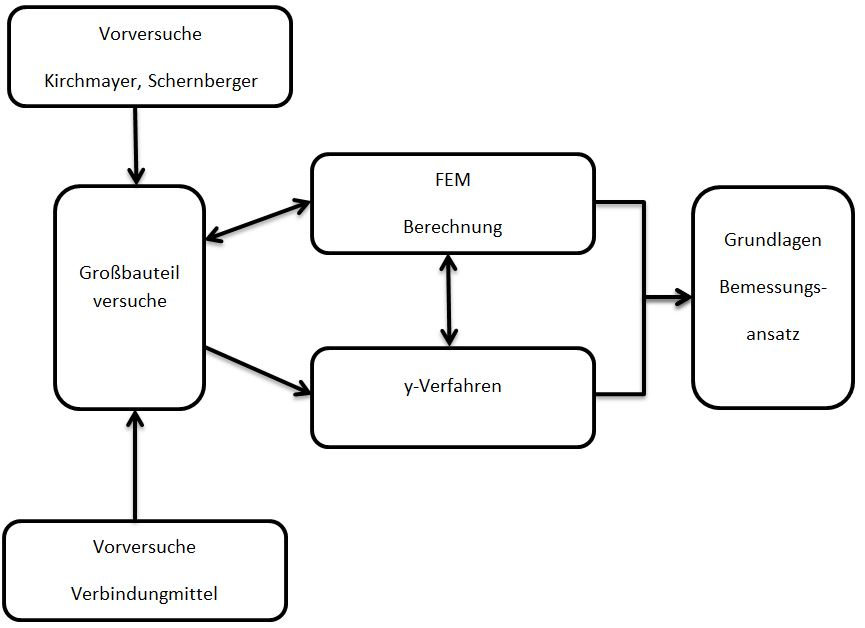
\includegraphics[scale=0.7]{Einleitung/ablauforganigramm.JPG}
\caption{Ablauforganigramm der Diplomarbeit}
\end{center}
\end{figure}




\section{Zusammenfassung der Kapitel}

\begin{enumerate}
\item Zusammenfassung von Vorarbeit 
\item Ermittlung der mechanischen Eigenschaften der Verbindungsmittel
\item Versuchaufbau und Durchführung
\item Beschreibung und Auswertung der Großbauteilversuche
\item Beschreibung der Berechnungsverfahren
\item Vergleich Berechnung Versuche und Berechnungen
\item wirtschaftliche Untersuchungen

\end{enumerate}